\section{Results: CKA Regularisation}
\label{sec:res_cka}

\begin{table}[tbp]
  \centering
  \caption{LoRA with and without the decoder CKA loss, both trained with 20\,px jitter, tight-box evaluation, mean $\pm$ std over three seeds; $\Delta$HD95 in pixels. $p$: paired Wilcoxon over per-image Dice at 20\,px evaluation jitter, pairs matched on seed and image, Holm-corrected.}
  \label{tab:cka}
  \begin{tabular}{lcccrr}
\toprule
Dataset & no-CKA Dice & CKA Dice & $\Delta$Dice & $\Delta$HD95 (px) & $p$ (Holm) \\
\midrule
ISIC (ID) & 0.949 $\pm$ 0.002 & 0.952 $\pm$ 0.002 & +0.003 & -0.3 & $<$0.001 \\
PH2 (near-OOD) & 0.951 $\pm$ 0.001 & 0.954 $\pm$ 0.002 & +0.003 & -0.4 & $<$0.001 \\
BUSI (far-OOD) & 0.774 $\pm$ 0.032 & 0.826 $\pm$ 0.008 & +0.051 & -96.1 & $<$0.001 \\
CBIS-DDSM (far-OOD) & 0.437 $\pm$ 0.095 & 0.541 $\pm$ 0.095 & +0.104 & -152.4 & $<$0.001 \\
\bottomrule
\end{tabular}

\end{table}

\paragraph{Multi-seed effect.}
Table~\ref{tab:cka} gives the main comparison. The decoder CKA loss leaves in-domain and near-OOD Dice within 0.003 and raises far-OOD Dice by 0.051 on BUSI and 0.104 on CBIS-DDSM, with HD95 falling by 96 and 152 pixels: the regulariser removes the boundary failures of unregularised LoRA rather than small overlap losses. The BUSI gain is stable across seeds (std 0.008 against 0.032 without the loss); on CBIS-DDSM the seed spread is large for both models (std 0.095) but the gain holds in every seed, and the paired test is significant on all four datasets with a median per-image gain of 0.088 on CBIS-DDSM. With tight-box training the loss gives smaller same-signed gains (0.033, 0.027; seed 0); with rand100 training it hurts (0.059 and 0.032 lower), so the two regularisers compound at mild jitter and conflict under heavy jitter.

\begin{figure}[tbp]
  \centering
  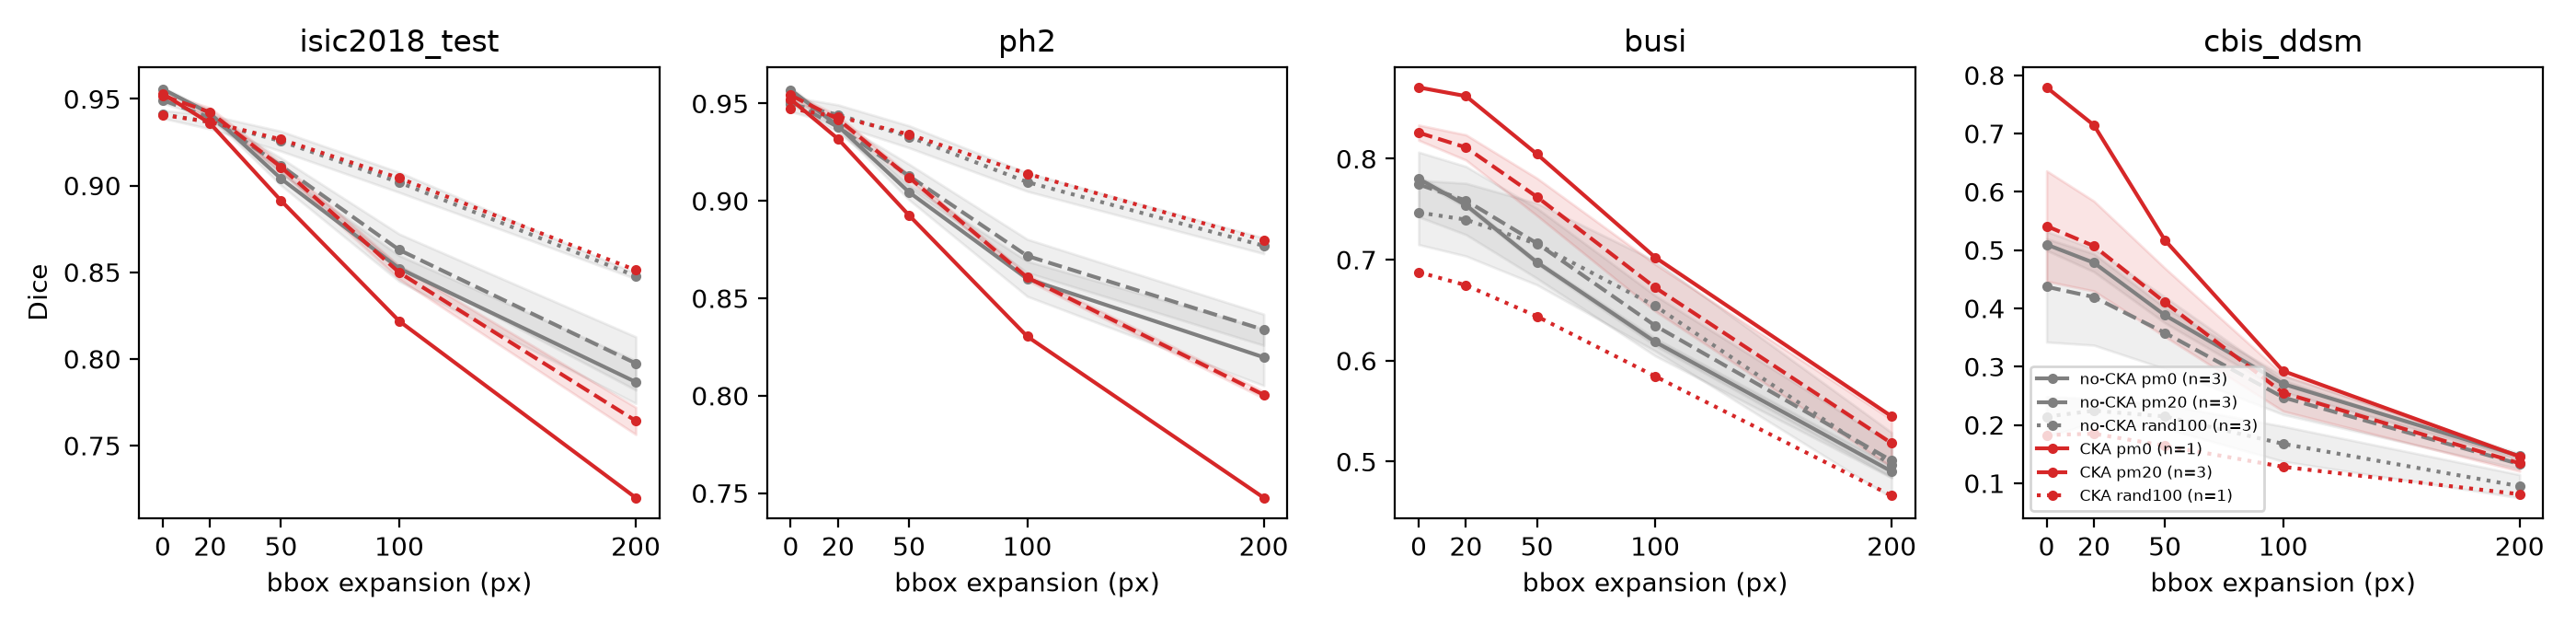
\includegraphics[width=0.86\linewidth]{figures/robustness_six_curves.png}
  \caption{Dice against outward box expansion for LoRA with (red) and without (grey) the decoder CKA loss under three training regimes: tight (solid), 20\,px jitter (dashed), random jitter up to 100\,px (dotted). Bands: one std over three seeds where available.}
  \label{fig:curves}
\end{figure}

\paragraph{Prompt robustness.}
In Fig.~\ref{fig:curves} the regularised pm20 model is the best of the six on both far-OOD sets at every expansion, with an advantage that narrows as boxes loosen: the paired gain on BUSI is 0.053, 0.046, 0.038 and 0.017 at 20, 50, 100 and 200\,px, and on CBIS-DDSM 0.088, 0.052, 0.008 and not significant. On the dermoscopy sets the sign flips beyond 50\,px (0.013 lower at 100\,px, 0.033 at 200\,px, $p < 10^{-20}$): anchoring to a base trained with tight boxes inherits its sensitivity to loose boxes in-domain. The rand100 regime is the other side of the trade, buying in-domain prompt robustness at a far-OOD price that the CKA loss makes worse.

\begin{figure}[tbp]
  \centering
  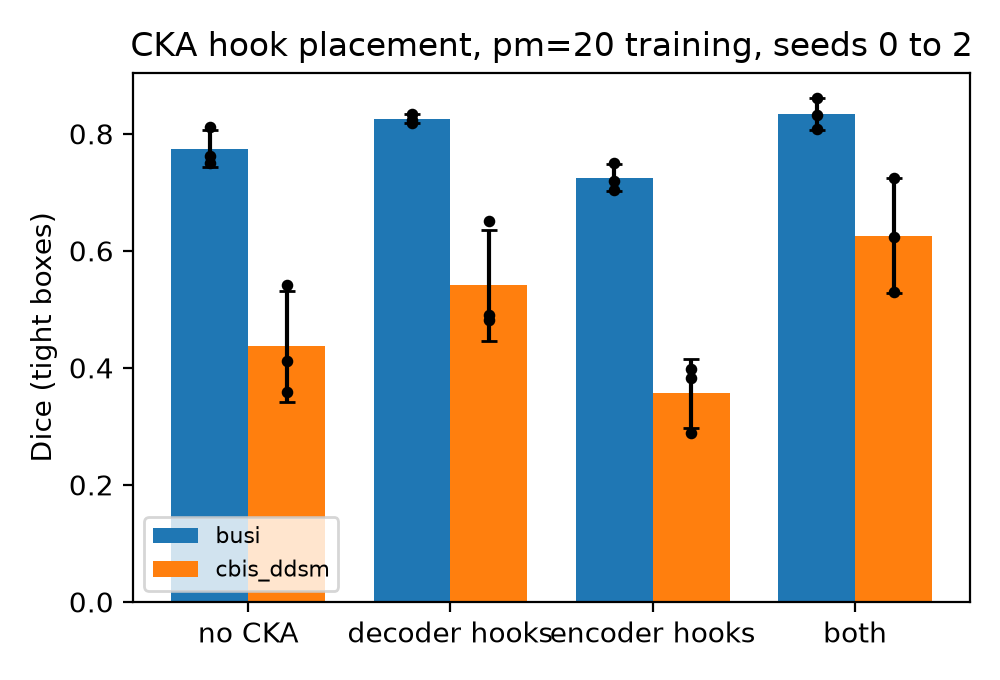
\includegraphics[width=0.36\linewidth]{figures/hook_ablation.png}
  \caption{Hook placement (LoRA, 20\,px training, tight-box evaluation): far-OOD Dice with no regulariser, decoder hooks, encoder hooks, and both; bars are means over seeds 0 to 2 with one std, dots the individual seeds.}
  \label{fig:hooks}
\end{figure}

\paragraph{Where the anchor must be.}
Figure~\ref{fig:hooks} separates the two halves of the model over three seeds. With the loss on encoder activations alone, far-OOD Dice falls below the unregularised baseline in every seed, to $0.725 \pm 0.023$ on BUSI and $0.357 \pm 0.059$ on CBIS-DDSM (paired per-image loss 0.037 and 0.055, $p < 10^{-4}$), at unchanged in-domain Dice. Decoder hooks give the gains of Table~\ref{tab:cka}. Anchoring both is best: $0.834 \pm 0.027$ and $0.626 \pm 0.098$, a paired gain over decoder hooks of 0.010 and 0.088 (median 0.062, $p < 10^{-4}$) and over no regulariser of 0.062 and 0.175, with 76 percent of CBIS-DDSM images improved, for a 0.003 in-domain cost. The seed spread on CBIS-DDSM is large for every arm (the best single run, seed 0 with both hooks, reaches 0.725; two independent trainings of the tight-box decoder-hook configuration reached 0.536 and 0.779), so we report paired statistics rather than best seeds. The decoder is the locus, and the encoder anchor helps only once the decoder is anchored too.

\paragraph{A second mammography source.}
On DMID, which no model or probe has seen (269 images, tight boxes, table in the supplement), LoRA falls from a zero-shot 0.637 to 0.402 and VPT to 0.53 and 0.57, while decoder-only, encoder-only LoRA and full fine-tuning reach 0.727 to 0.733; the decoder anchor lifts LoRA to 0.697 (tight-box training) and 0.651 (both hooks), encoder hooks alone give 0.366. Every comparison matches CBIS-DDSM.
